\section{桥接与装饰者}

\subsection{桥接模式}

\subsubsection{模式动机}
设想如果要绘制矩形、圆形、椭圆、正方形,我们至少需要4个形状类,但是如果绘制的图形需要具有不同的颜色,如红色、绿色、蓝色等,此时至少有如下两种设计方案:
\begin{figure}[H]
    \vspace{-0.5em}
	\centering
	\includegraphics[width=0.95\textwidth]{images/桥接模式动机.pdf}
    \vspace{-1em}
\end{figure}
\begin{itemize}
    \item 第一种设计方案是为每一种形状都提供一套各种颜色的版本。
    \item 第二种设计方案是根据实际需要对形状和颜色进行组合。
\end{itemize}

对于有两个变化维度(即两个变化的原因)的系统,采用方案二来进行设计系统中类的个数更少,且系统扩展更为方便。设计方案二即是桥接模式的应用。桥接模式\textbf{将继承关系转换为关联关系,从而降低了类与类之间的耦合,减少了代码编写量}。

\subsubsection{模式定义}
桥接模式(Bridge Pattern):将抽象部分与它的实现部分分离,使它们都可以独立地变化。它是一种对象结构型模式,又称为柄体(Handle and Body)模式或接口(Interface)模式。

\subsubsection{模式结构}
桥接模式包含如下角色:
\vspace{-0.8em}
\begin{multicols}{2}
    \begin{itemize}
        \item Abstraction:抽象类
        \item RefinedAbstraction:扩充抽象类
        \item Implementor:实现类接口
        \item ConcreteImplementor:具体实现类
    \end{itemize}
\end{multicols}
\vspace{-1em}

\begin{figure}[H]
    \vspace{-0.5em}
	\centering
	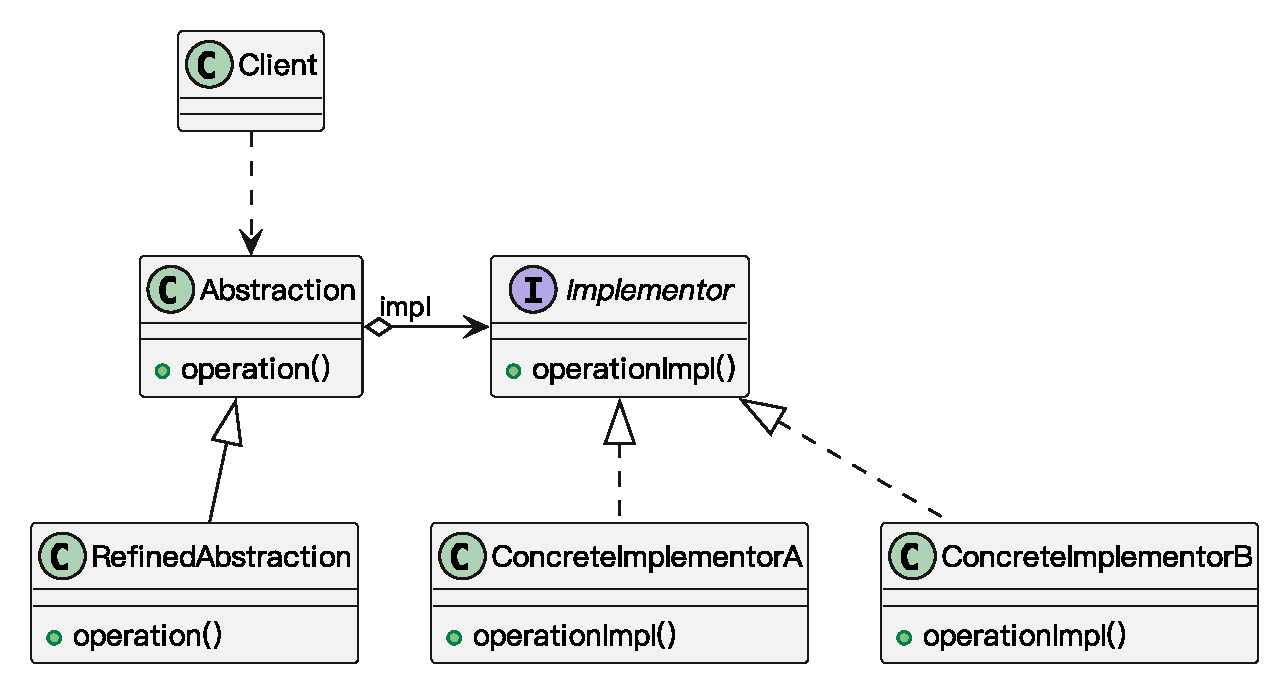
\includegraphics[width=0.62\textwidth]{images/桥接模式结构.eps}
    \vspace{-1em}
\end{figure}

\subsubsection{模式分析}
理解桥接模式,重点需要理解如何将\textbf{抽象化}(Abstraction)与\textbf{实现化}(Implementation)\textbf{脱耦},使得二者可以独立地变化。
\begin{itemize}
    \item \textbf{抽象化}:抽象化就是忽略一些信息,把不同的实体当作同样的实体对待。在面向对象中,\textbf{将对象的共同性质抽取出来形成类}的过程即为抽象化的过程。
    \item \textbf{实现化}:\textbf{针对抽象化给出的具体实现},就是实现化,抽象化与实现化是一对互逆的概念,实现化产生的对象比抽象化更具体,是对抽象化事物的进一步具体化的产物。
    \item \textbf{脱耦}:脱耦就是\textbf{将抽象化和实现化之间的耦合解脱开},或者说是\textbf{将它们之间的强关联改换成弱关联,将两个角色之间的继承关系改为关联关系}。桥接模式中的所谓脱耦,就是指在一个软件系统的抽象化和实现化之间使用关联关系(组合或者聚合关系)而不是继承关系,从而使两者可以相对独立地变化,这就是桥接模式的用意。
\end{itemize}

桥接模式典型代码:
\begin{figure}[H]
    \vspace{-0.5em}
	\centering
	\includegraphics[width=0.95\textwidth]{images/桥接模式典型代码.pdf}
    \vspace{-1em}
\end{figure}

\subsubsection{模式实例}
模拟毛笔:现需要提供大中小3种型号的画笔,能够绘制5种不同颜色,如果使用蜡笔,我们需要准备$3\times 5=15$支蜡笔,也就是说必须准备15个具体的蜡笔类。而如果使用毛笔的话,只需要3种型号的毛笔,外加5个颜料盒,用$3+5=8$个类就可以实现15支蜡笔的功能。本实例使用桥接模式来模拟毛笔的使用过程。
\begin{figure}[H]
    \vspace{-0.5em}
	\centering
	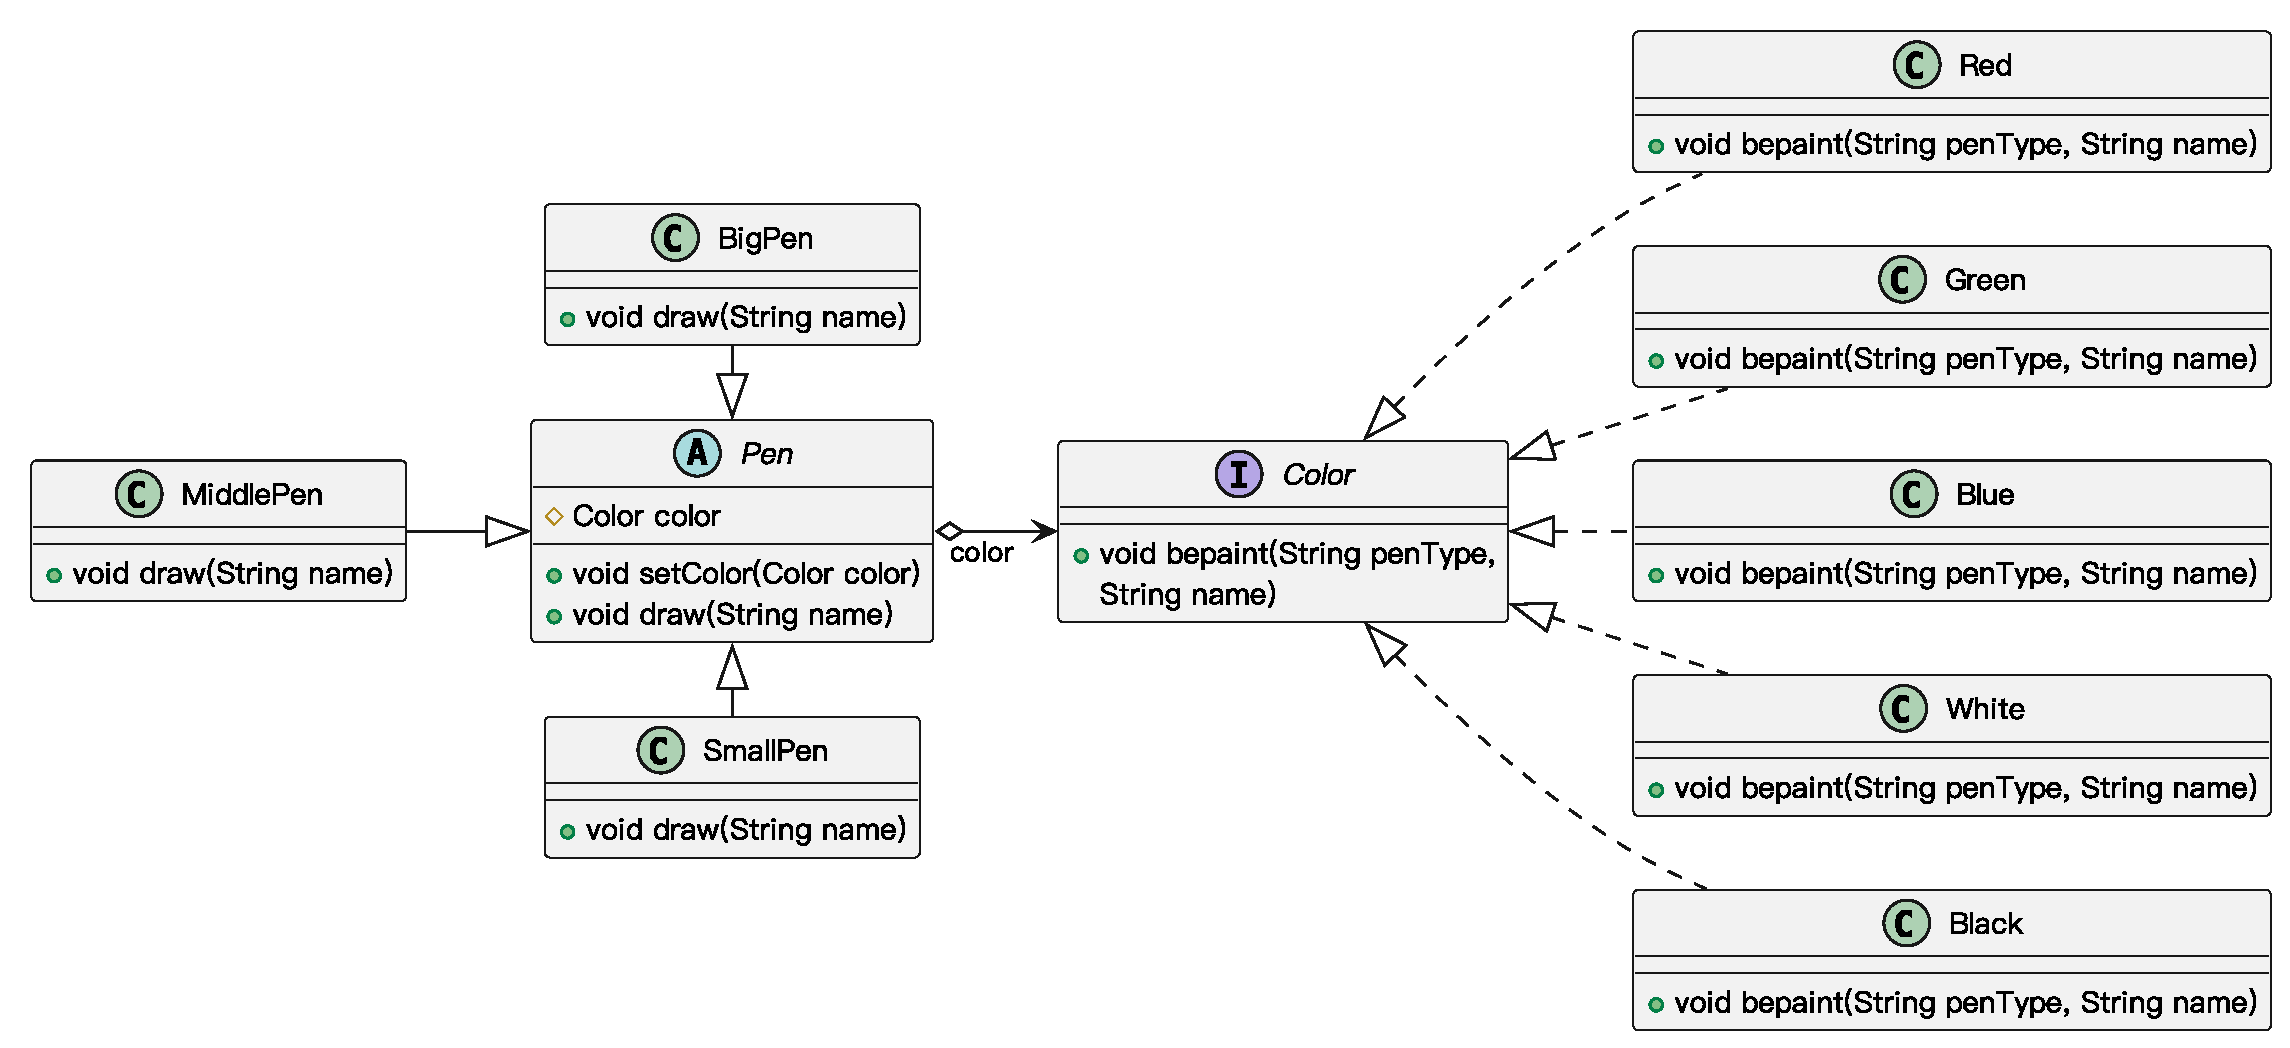
\includegraphics[width=\textwidth]{images/桥接模式实例1.eps}
    \vspace{-1em}
\end{figure}

跨平台视频播放器:如果需要开发一个跨平台视频播放器,可以在不同操作系统平台(如Windows、Linux、Unix等)上播放多种格式的视频文件,常见的视频格式包括MPEG、RMVB、AVI、WMV等。现使用桥接模式设计该播放器。
\begin{figure}[H]
    \vspace{-0.5em}
	\centering
	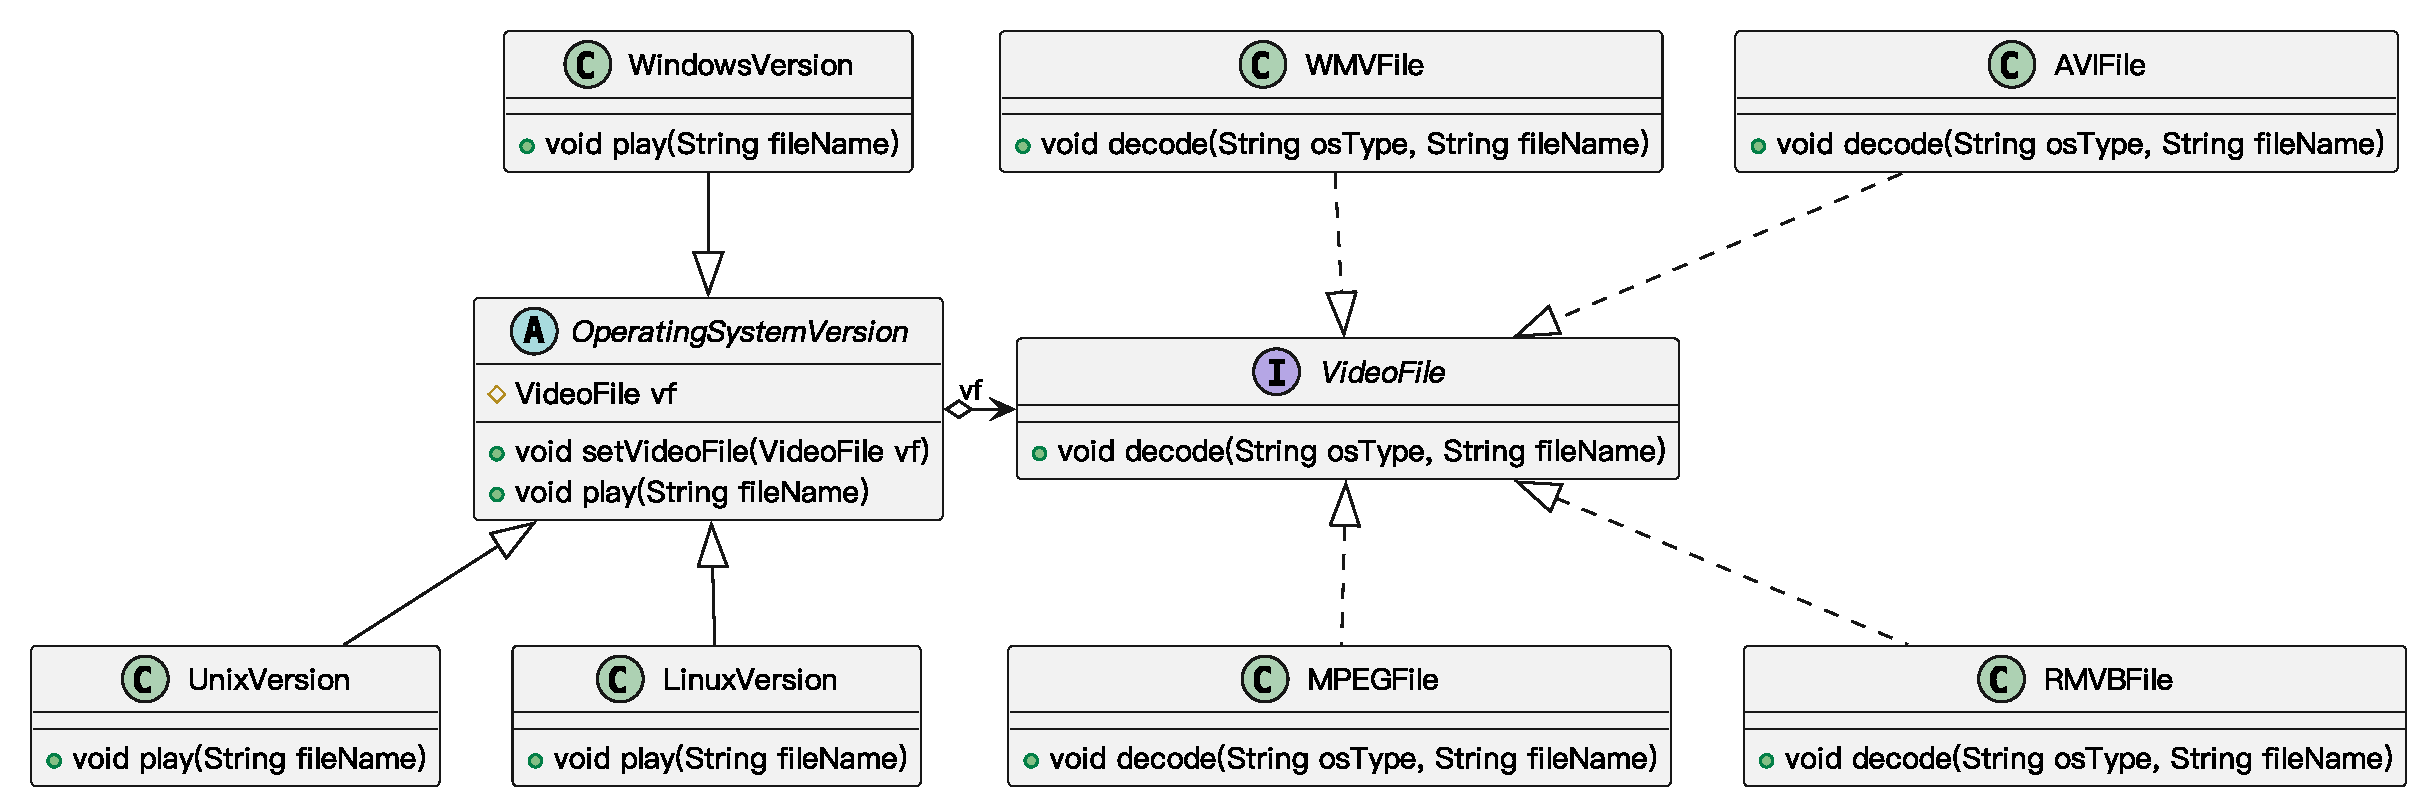
\includegraphics[width=\textwidth]{images/桥接模式实例2.eps}
    \vspace{-1em}
\end{figure}

\subsubsection{模式优缺点}
桥接模式的优点:
\begin{itemize}
    \item 分离抽象接口及其实现部分。
    \item 桥接模式有时类似于多继承方案,但是多继承方案违背了类的单一职责原则(即一个类只有一个变化的原因),复用性比较差,而且多继承结构中类的个数非常庞大,\textbf{桥接模式是比多继承方案更好的解决方法}。
    \item 桥接模式\textbf{提高了系统的可扩充性},在两个变化维度中任意扩展一个维度,都不需要修改原有系统。
    \item 实现细节对客户透明,可以对用户隐藏实现细节。
\end{itemize}

桥接模式的缺点:
\begin{itemize}
    \item 桥接模式的引入会\textbf{增加系统的理解与设计难度},由于聚合关联关系建立在抽象层,要求开发者针对抽象进行设计与编程。
    \item 桥接模式要求正确识别出系统中两个独立变化的维度,因此\textbf{其使用范围具有一定的局限性}。
\end{itemize}

\subsubsection{模式适用环境}
在以下情况下可以使用桥接模式:
\begin{itemize}
    \item 如果一个系统\textbf{需要在构件的抽象化角色和具体化角色之间增加更多的灵活性,避免在两个层次之间建立静态的继承联系},通过桥接模式可以使它们在抽象层建立一个关联关系。
    \item \textbf{抽象化角色和实现化角色可以以继承的方式独立扩展而互不影响},在程序运行时可以动态将一个抽象化子类的对象和一个实现化子类的对象进行组合,即系统需要对抽象化角色和实现化角色进行动态耦合。
    \item 一个类\textbf{存在两个独立变化的维度},且这两个维度都需要进行扩展。
    \item 虽然在系统中使用继承是没有问题的,但是由于抽象化角色和具体化角色需要独立变化,设计要求需要独立管理这两者。
    \item 对于那些\textbf{不希望使用继承或因为多层次继承导致系统类的个数急剧增加的系统},桥接模式尤为适用。
\end{itemize}

\subsubsection{模式应用}
\ding{172} Java语言通过Java虚拟机实现了平台的无关性。
\begin{figure}[H]
    \vspace{-0.5em}
	\centering
	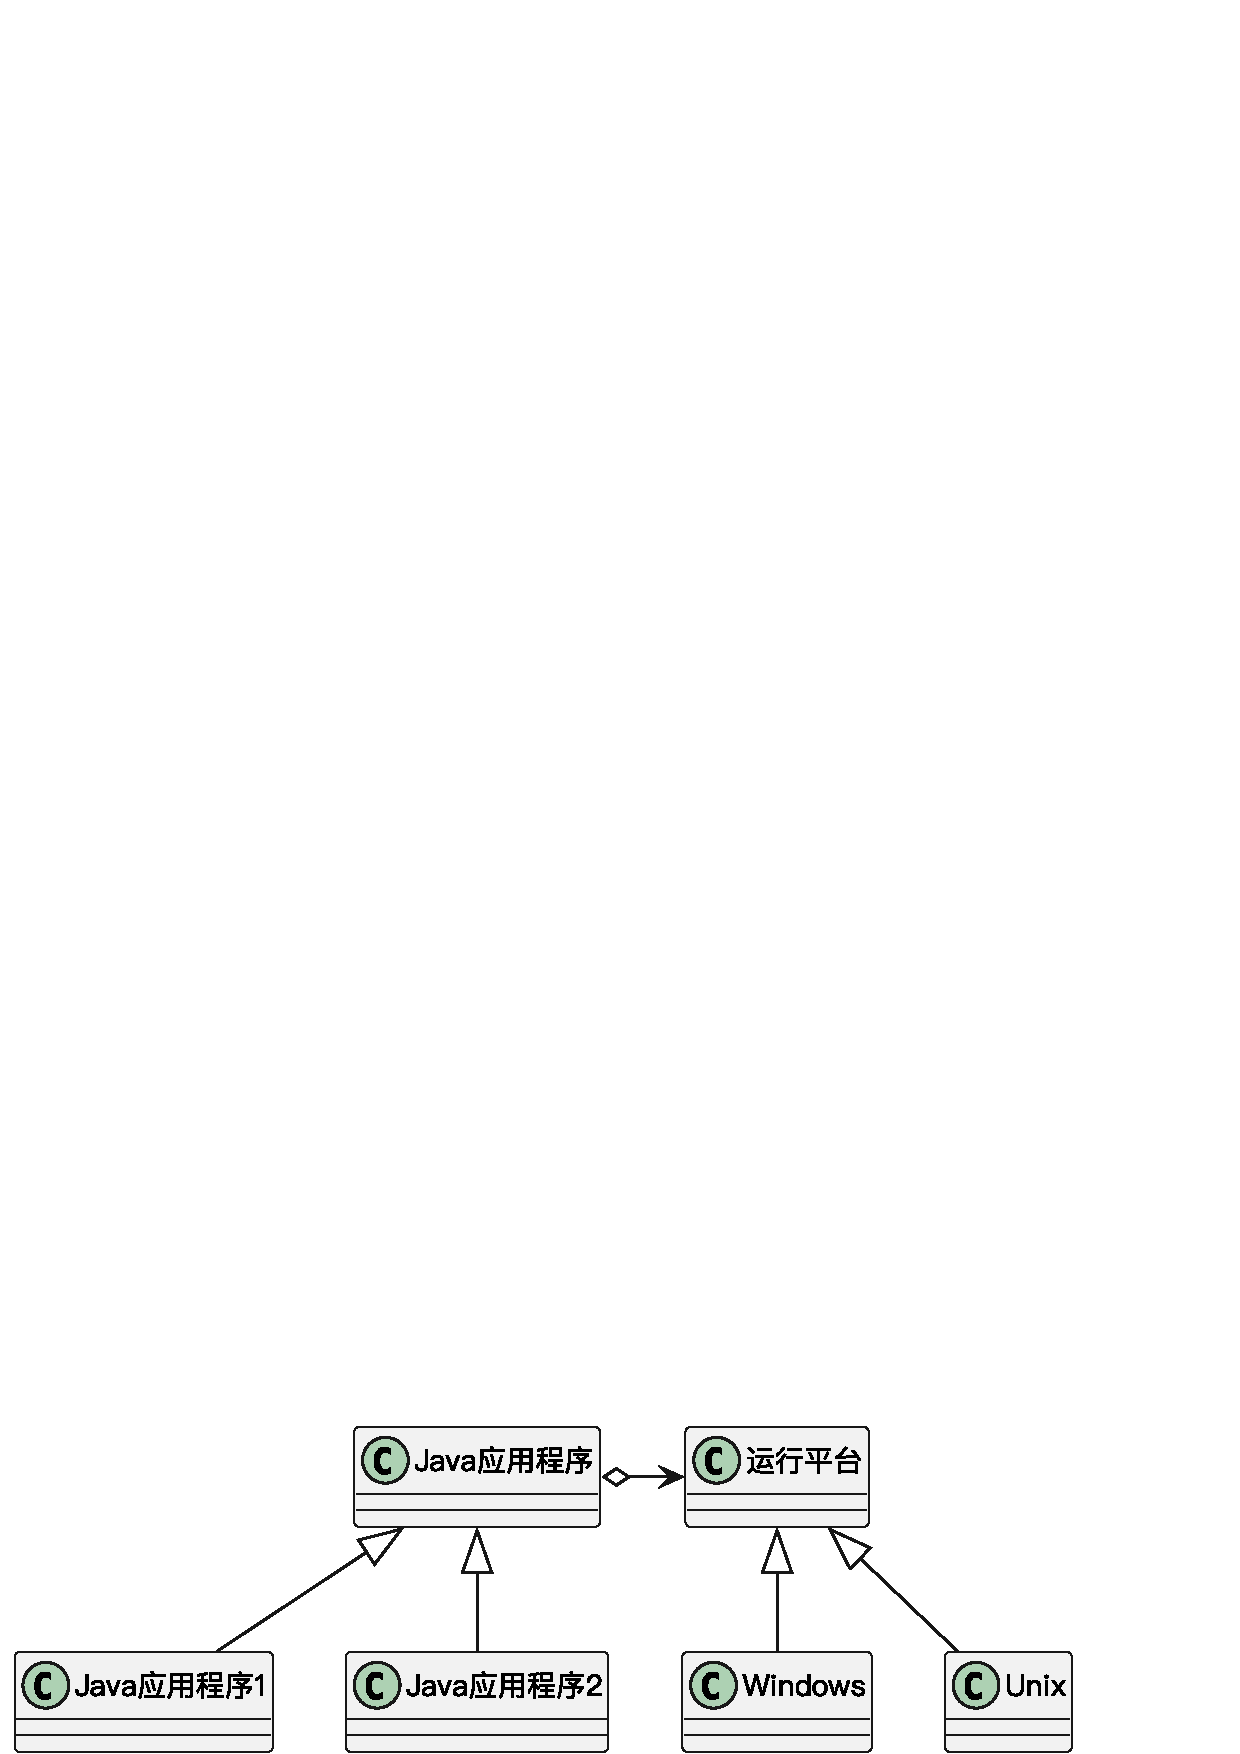
\includegraphics[width=0.65\textwidth]{images/桥接模式应用1.pdf}
    \vspace{-1em}
\end{figure}

\ding{173} 一个Java桌面软件总是带有所在操作系统的视感(LookAndFeel),如果一个Java软件是在Unix系统上开发的,那么开发人员看到的是Motif用户界面的视感;在Windows上面使用这个系统的用户看到的是Windows用户界面的视感;而一个在Macintosh上面使用的用户看到的则是Macintosh用户界面的视感,Java语言是通过所谓的Peer架构做到这一点的。Java为AWT中的每一个GUI构件都提供了一个Peer构件,\textbf{在AWT中的Peer架构就使用了桥接模式}。

\ding{174} JDBC驱动程序也是桥接模式的应用之一。使用JDBC驱动程序的应用系统就是抽象角色,而所使用的数据库是实现角色。\textbf{一个JDBC驱动程序可以动态地将一个特定类型的数据库与一个Java应用程序绑定在一起,从而实现抽象角色与实现角色的动态耦合}。

\subsubsection{模式扩展}
\paragraph*{适配器模式与桥接模式的联用}~{} \par
桥接模式和适配器模式用于设计的不同阶段,\textbf{桥接模式用于系统的初步设计},对于存在两个独立变化维度的类可以将其分为抽象化和实现化两个角色,使它们可以分别进行变化;而在初步设计完成之后,\textbf{当发现系统与已有类无法协同工作时,可以采用适配器模式}。但有时候在设计初期也需要考虑适配器模式,特别是那些涉及到大量第三方应用接口的情况。
\begin{figure}[H]
    \vspace{-0.5em}
	\centering
	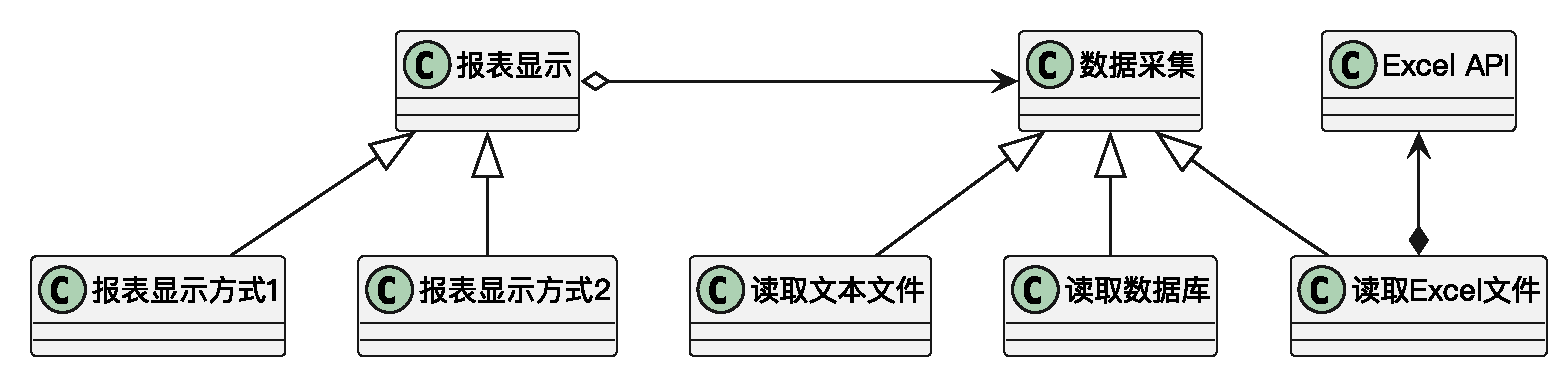
\includegraphics[width=0.85\textwidth]{images/桥接模式拓展.eps}
    \vspace{-1em}
\end{figure}

\subsection{装饰模式}

\subsubsection{模式动机}
一般有两种方式可以实现给一个类或对象增加行为:
\begin{itemize}
    \item \textbf{继承机制}:使用继承机制是给现有类添加功能的一种有效途径,通过继承一个现有类可以使得子类在拥有自身方法的同时还拥有父类的方法。但是这种方法是静态的,用户不能控制增加行为的方式和时机。
    \item \textbf{关联机制}:即将一个类的对象嵌入另一个对象中,由另一个对象来决定是否调用嵌入对象的行为以便扩展自己的行为。
\end{itemize}

装饰模式以\textbf{对客户透明的方式动态地给一个对象附加上更多的责任},换言之,客户端并不会觉得对象在装饰前和装饰后有什么不同。装饰模式可以\textbf{在不需要创造更多子类的情况下,将对象的功能加以扩展}。这就是装饰模式的模式动机。

\subsubsection{模式定义}
装饰模式(Decorator Pattern) :动态地给一个对象增加一些额外的职责(Responsibility),就增加对象功能来说,装饰模式比生成子类实现更为灵活。其别名也可以称为包装器(Wrapper),与适配器模式的别名相同,但它们适用于不同的场合。根据翻译的不同,装饰模式也有人称之为“油漆工模式”,它是一种对象结构型模式。

\subsubsection{模式结构}
装饰模式包含如下角色:
\vspace{-0.8em}
\begin{multicols}{2}
    \begin{itemize}
        \item Component:抽象构件
        \item ConcreteComponent:具体构件
        \item Decorator:抽象装饰类
        \item ConcreteDecorator:具体装饰类
    \end{itemize}
\end{multicols}
\vspace{-1em}

\begin{figure}[H]
    \vspace{-0.5em}
	\centering
	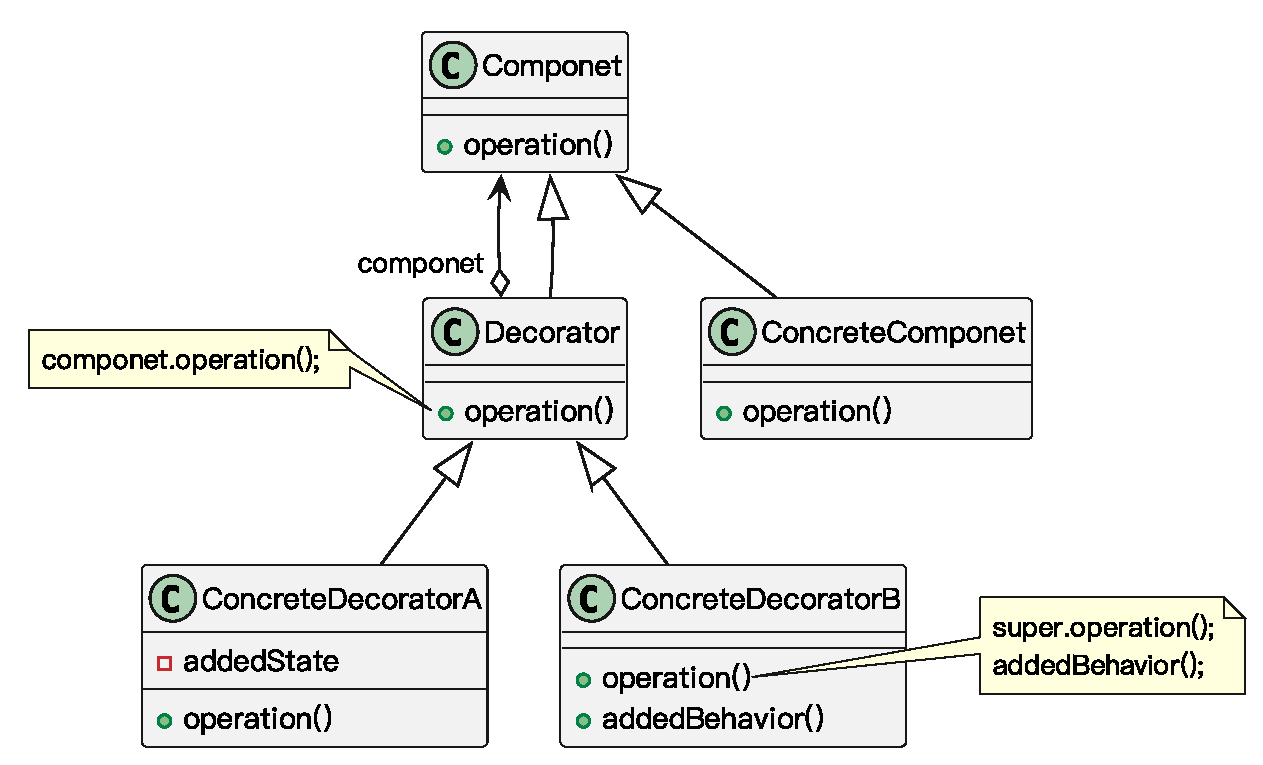
\includegraphics[width=0.75\textwidth]{images/装饰模式结构.eps}
    \vspace{-1em}
\end{figure}

与继承关系相比,关联关系的主要优势在于\textbf{不会破坏类的封装性},而且\textbf{继承是一种耦合度较大的静态关系,无法在程序运行时动态扩展}。在软件开发阶段,关联关系虽然不会比继承关系减少编码量,但是到了软件维护阶段,由于关联关系使系统具有较好的\textbf{松耦合性},因此使得\textbf{系统更加容易维护}。当然,关联关系的缺点是\textbf{比继承关系要创建更多的对象}。

使用装饰模式来实现扩展比继承更加灵活,它\textbf{以对客户透明的方式动态地给一个对象附加更多的责任}。装饰模式可以在不需要创造更多子类的情况下,将对象的功能加以扩展。

装饰模式示例代码:
\begin{figure}[H]
    \vspace{-0.5em}
	\centering
	\includegraphics[width=0.98\textwidth]{images/装饰模式典型代码.pdf}
    \vspace{-1em}
\end{figure}

\subsubsection{模式实例}
变形金刚:变形金刚在变形之前是一辆汽车,它可以在陆地上移动。当它变成机器人之后除了能够在陆地上移动之外,还可以说话;如果需要,它还可以变成飞机,除了在陆地上移动还可以在天空中飞翔。
\begin{figure}[H]
    \vspace{-0.5em}
	\centering
	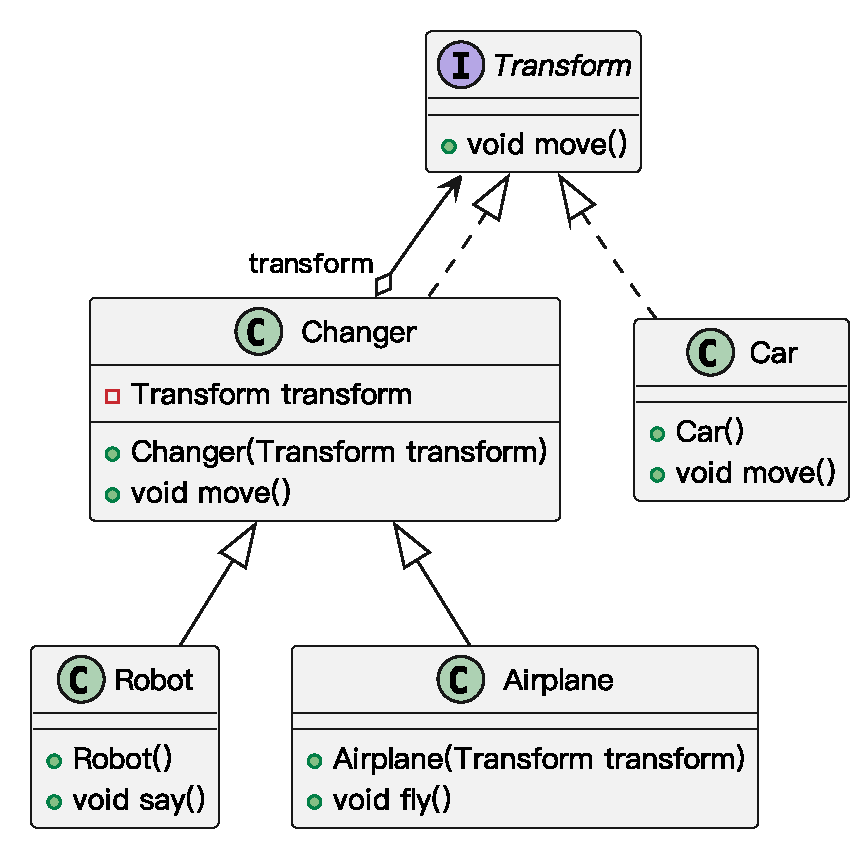
\includegraphics[width=0.47\textwidth]{images/装饰模式实例1.eps}
    \vspace{-1em}
\end{figure}

多重加密系统:某系统提供了一个数据加密功能,可以对字符串进行加密。最简单的加密算法通过对字母进行移位来实现,同时还提供了稍复杂的逆向输出加密,还提供了更为高级的求模加密。用户先使用最简单的加密算法对字符串进行加密,如果觉得还不够可以对加密之后的结果使用其他加密算法进行二次加密,当然也可以进行第三次加密。现使用装饰模式设计该多重加密系统。
\begin{figure}[H]
    \vspace{-0.5em}
	\centering
	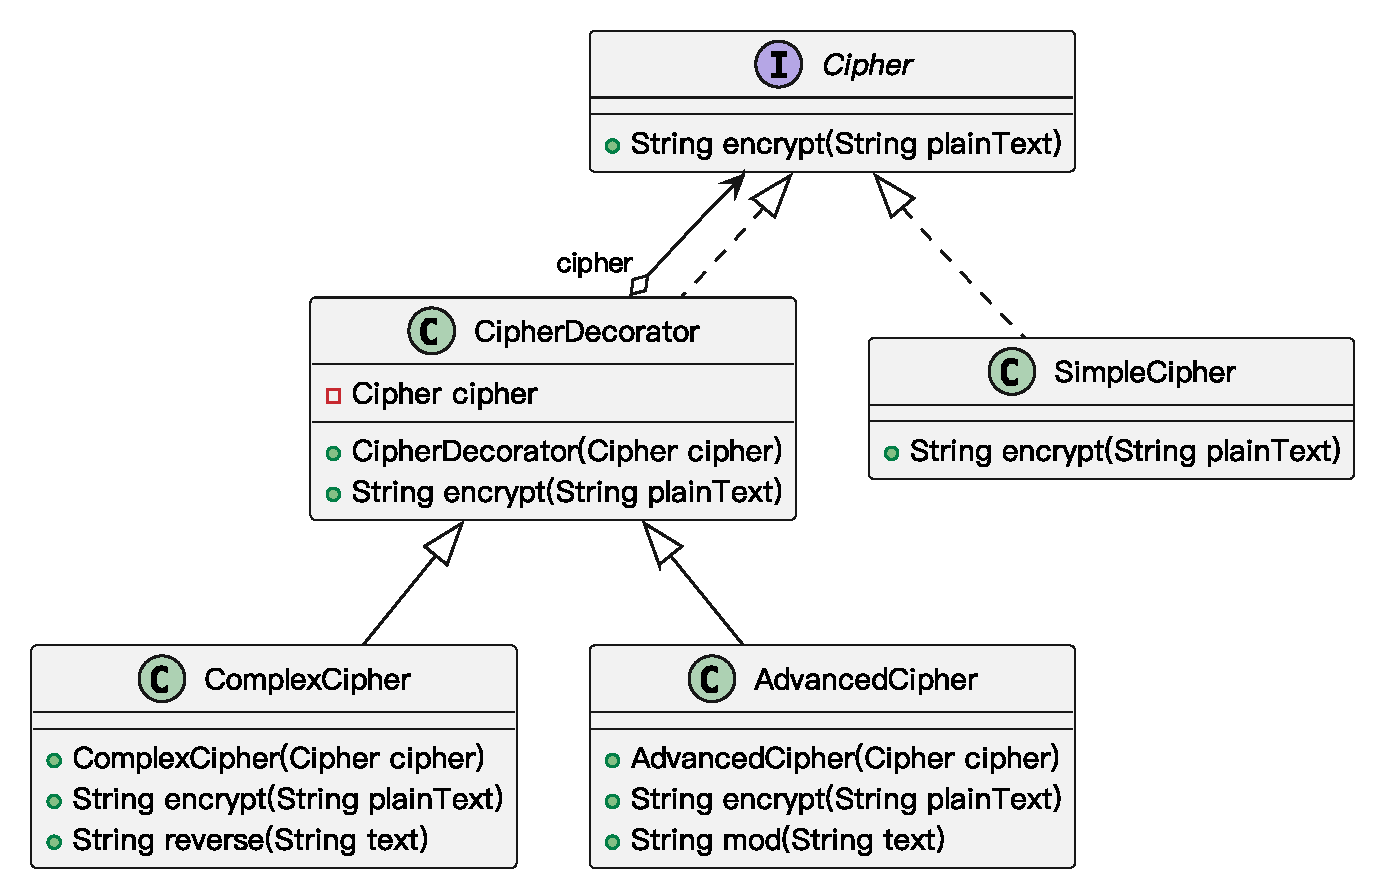
\includegraphics[width=0.7\textwidth]{images/装饰模式实例2.eps}
    \vspace{-1em}
\end{figure}

\subsubsection{模式优缺点}
装饰模式的优点:
\begin{itemize}
    \item 装饰模式与继承关系的目的都是要扩展对象的功能,但是\textbf{装饰模式可以提供比继承更多的灵活性}。
    \item 可以\textbf{通过一种动态的方式来扩展一个对象的功能},通过配置文件可以在运行时选择不同的装饰器,从而实现不同的行为。
    \item \textbf{通过使用不同的具体装饰类以及这些装饰类的排列组合,可以创造出很多不同行为的组合}。可以使用多个具体装饰类来装饰同一对象,得到功能更为强大的对象。
    \item \textbf{具体构件类与具体装饰类可以独立变化},用户可以根据需要增加新的具体构件类和具体装饰类,在使用时再对其进行组合,原有代码无须改变,符合“开闭原则”。
\end{itemize}

装饰模式的缺点:
\begin{itemize}
    \item 使用装饰模式进行系统设计时\textbf{将产生很多小对象},这些对象的区别在于它们之间相互连接的方式有所不同,而不是它们的类或者属性值有所不同,同时还将产生很多具体装饰类。这些装饰类和小对象的产生将增加系统的复杂度,加大学习与理解的难度。
    \item 这种比继承更加灵活机动的特性,也同时意味着\textbf{装饰模式比继承更加易于出错,排错也很困难,对于多次装饰的对象,调试时寻找错误可能需要逐级排查,较为烦琐}。
\end{itemize}

\subsubsection{模式适用环境}
在以下情况下可以使用装饰模式:
\begin{itemize}
    \item 在不影响其他对象的情况下,\textbf{以动态、透明的方式给单个对象添加职责}。
    \item 需要\textbf{动态地给一个对象增加功能},这些功能也可以\textbf{动态地被撤销}。
    \item \textbf{当不能采用继承的方式对系统进行扩充或者采用继承不利于系统扩展和维护时}。不能采用继承的情况主要有两类:第一类是系统中存在大量独立的扩展,为支持每一种组合将产生大量的子类,使得子类数目呈爆炸性增长;第二类是因为类定义不能继承(如final类)。
\end{itemize}

\subsubsection{模式应用}
\ding{172} 在javax.swing包中,可以通过装饰模式动态给一些构件增加新的行为或改善其外观显示。如\sverb|JList|\;构件本身并不支持直接滚动,即没有滚动条,要创建可以滚动的列表,可以使用如下代码实现:
\begin{lstlisting}
JList list = new JList();
JScrollPane sp = new JScrollPane(list);  
\end{lstlisting}

\ding{173} 装饰模式在JDK中最经典的实例是Java IO。以\sverb|InputStream|\;为例:
\begin{figure}[H]
	\centering
    \vspace{-0.5em}
	\subfloat{
	\begin{minipage}[c]{0.53\linewidth}
		\centering
		\includegraphics[width=0.99\linewidth]{images/装饰模式应用1.pdf}
	\end{minipage}
	}
    \subfloat{
    \begin{minipage}[c]{0.44\linewidth}
        \centering
        \includegraphics[width=0.99\linewidth]{images/装饰模式应用2.pdf}
    \end{minipage}
    }
	\centering
    \vspace{-1em}
\end{figure}

\subsubsection{模式扩展}
\paragraph*{装饰模式的简化}~{} \par
需要注意的问题:
\begin{itemize}
    \item \textbf{一个装饰类的接口必须与被装饰类的接口保持相同},对于客户端来说无论是装饰之前的对象还是装饰之后的对象都可以一致对待。
    \item 尽量保持具体构件类\sverb|Component|\;作为一个“轻”类,也就是说\textbf{不要把太多的逻辑和状态放在具体构件类中},可以通过装饰类对其进行扩展。
    \item \textbf{如果只有一个具体构件类而没有抽象构件类,那么抽象装饰类可以作为具体构件类的直接子类。}
\end{itemize}
\begin{figure}[H]
    \vspace{-0.5em}
	\centering
	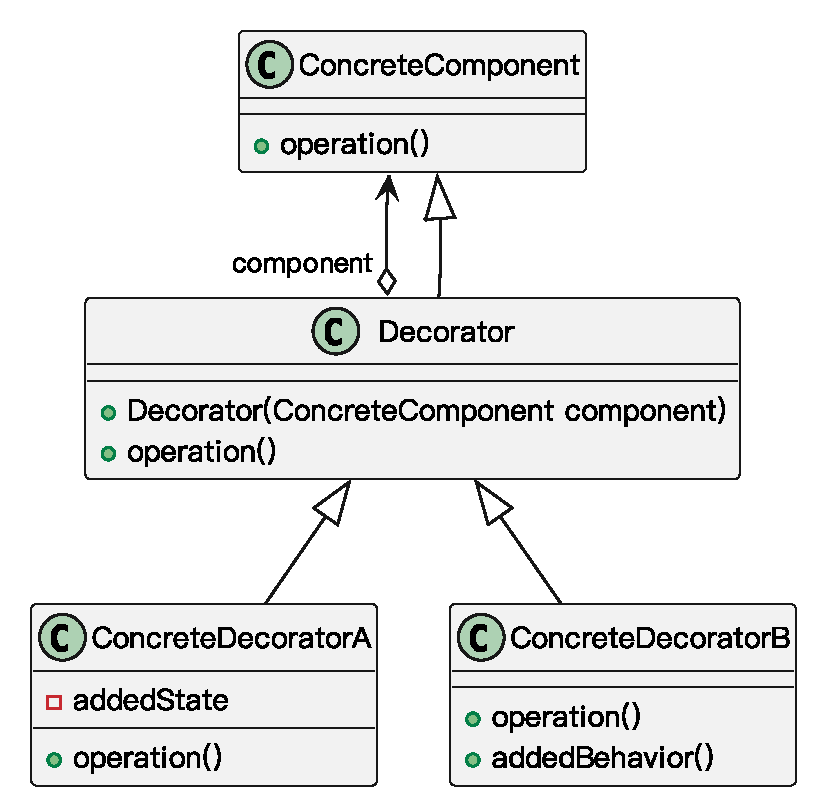
\includegraphics[width=0.45\textwidth]{images/装饰模式拓展.eps}
    \vspace{-1em}
\end{figure}


\paragraph*{透明装饰模式\footnote{如9.2.4模式示例中的多重加密系统例}}~{}  \par
在透明装饰模式中,要求客户端完全针对抽象编程,装饰模式的透明性要求客户端程序不应该声明具体构件类型和具体装饰类型,而应该全部声明为抽象构件类型。
\begin{lstlisting}
Cipher sc,cc,ac;
sc = new SimpleCipher();
cc = new ComplexCipher(sc);
ac = new AdvancedCipher(cc);
\end{lstlisting}

\paragraph*{半透明装饰模式\footnote{如9.2.4模式示例中的变形金刚例}}~{}  \par
半透明(semi-transparent)的装饰模式允许用户在客户端声明具体装饰者类型的对象,调用在具体装饰者中新增的方法。
\begin{lstlisting}
Transform camaro;
camaro = new Car();
camaro.move();
Robot bumblebee = new Robot(camaro);
bumblebee.move();
bumblebee.say();
\end{lstlisting}